%\bibliography{bibliography.bib} %The files containing all the articles and books you ever referenced. 

\chapter{Discussion}
\section{Scope}
The results of our HRV analyses must be interpreted within the scope and limitations of this study. Most importantly, our analyses were designed to simulate vegetation dynamics under a historic reference period. We chose the period from 1550 to 1850, representing the 300 years prior to European settlement, based on expert opinion \citetext{Hugh\ Safford,\ pers.\ comm.}(%20 September 2013)
. The arrival of European settlers to the Sierra Nevada was spurred primarily but not exclusively by the Gold Rush, and led to sweeping ecological changes that now have greatly altered many Sierran landscapes -- through fire suppression, grazing, road-building, timber cutting, recreation, and other activities \citep{Meyer2013,Safford2013}\todo{others?}. Climatically, this time frame does fall during the ``Little Ice Age.'' However, \citet{Safford2013} argues that vegetation change did not change substantially during the time. The period prior to European settlement, then, is a suitable reference condition against which we can compare current landscape structure and dynamics. Moreover, it is frequently used in the western United States as the historical reference period for restoration planning \citep{Safford2013}. The period is also up to several times the length of rotation periods identified for well-understood cover types within the project area. Finally, it is a timeframe for which we have a reasonable amount of specific information to enable us to model the system.

We do not argue here that the chosen reference period was a time of stasis, climatically, ecologically, or culturally. In Figure~\ref{pdsi} we illustrate how the Palmer Drought Severity index, a measure of climate variability, oscillates around an average value throughout the reference period. Multi-year droughts and El Ni\~no/La Ni\~na events also occurred over this time frame \citep{Meyer2013}. Ecologically, our historical period occurred during a very long-term (on the scale of thousands of years) shift to a warmer and drier climate, with an associated shift toward species more tolerant of such conditions, such as yellow pine species, and away from species like white fir, which prefer more mesic conditions. A slow shift toward more frequent fire was also taking place \citep{Safford2013}. Culturally, several Native American tribes were living throughout the project area during the reference period. Debate continues among scientists and researchers as to the extent to which those peoples managed vegetation through setting fires \citep{Safford2013}\todo{others?}. Because we lack empirical evidence to distinguish between lightning-caused and human-caused fires during the reference period, we decided not to exclude any fire frequency or rotation data on the basis of not being reflective of ``natural'' conditions.

We emphasize that our choice of reference periods does not suggest that it should be our goal in management to recreate all of the ecological conditions and dynamics of this period. Complete achievement of such a goal would be impossible, given the climatic, cultural, and ecological changes that have occurred in the last century. It also would be unacceptable socially, economically, and politically. Nor do we suggest that the reference period was completely ``natural'' or preferable in all ways to today’s landscape. 

\begin{wrapfigure}{r}{0.5\textwidth}
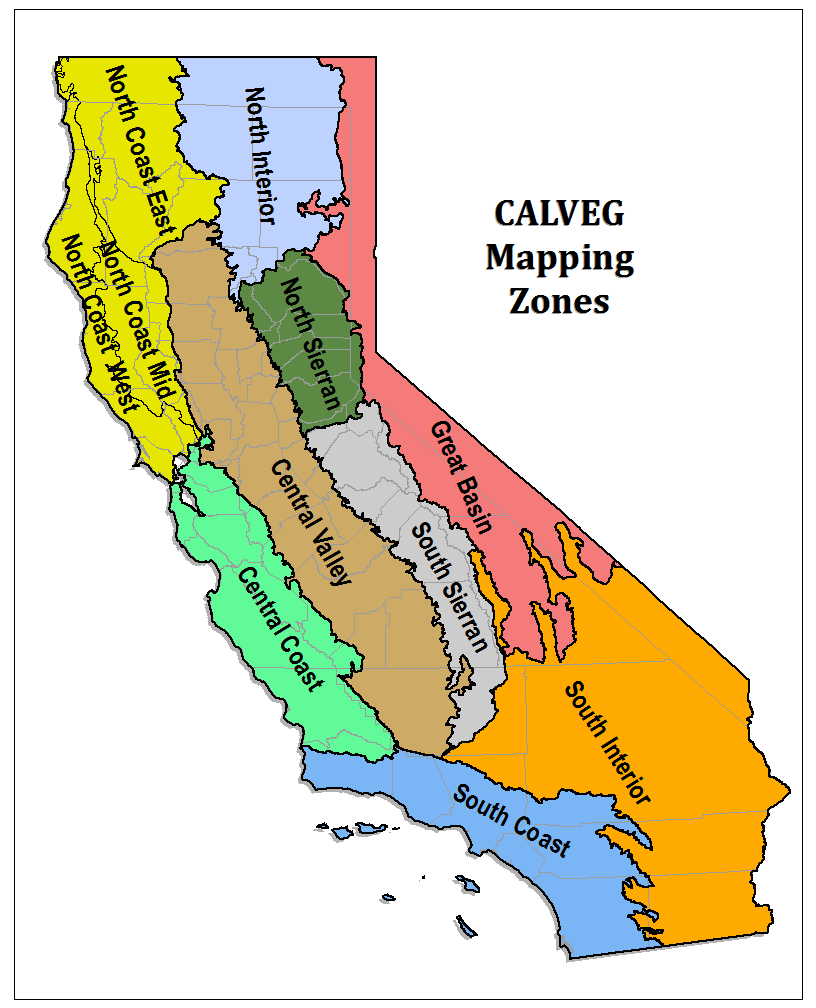
\includegraphics[width=0.48\textwidth]{images/CALVEGmappingzones.png}
\caption{\small CALVEG Mapping Zones. These zones meet U.S. Forest Service standard at national and regional levels. These ecological provinces are associated with dozens of vegetation alliances, which are used to classify vegetation in spatial data products.} 
\label{calveg}
\end{wrapfigure}

However, the reference period proposed will allow us to compare current conditions to a baseline set of data on ecosystem conditions (composition, configuration, and disturbance processes) ``to develop an idea of trend over time and idea of the level of depature of altered ecosystems from their ``natural'' state'' (Safford 2013). The results presented here will complement the Natural Range of Variability assessments compiled by the Forest Service's Pacific Southwest Region Ecology group \citep[e.g.,][]{Safford2013,Merriam2013,Meyer2013a,Meyer2013,Estes2013,Estes2013a,Gross2013}. An understanding of natural landscape structures and variability during this reference period also provides a basis for forest management policies and associated actions that seek to mimic natural disturbance patterns \cite{Romme2000,Buse2002}.

The spatial scope of our project extends generally to the the northern Sierra Nevada. When deciding on land cover types, including determining xeric and mesic subtypes, our focus was to best represent the project area and the surrounding landscape. We used the CALVEG Mapping Zone boundary for the ``North Sierra'' (Figure~\ref{calveg}) as our focus for defining vegetation and disturbance, including susceptibility, response to fire, and fire size and distribution. The model could be applied, with some revision, to the east-side of the Sierra Nevada, or to the southern mountains.

\section{Limitations}

Because our study relied on the use of computer models, it is imperative that the limitations of these models be understood before applying the results in a management context. Here, we discuss several important limitations, some general to the modeling approach employed here and some specific to how we parameterized these models for application in the northern Sierra Nevada.

First, while it is important to recognize the many advantages of models, it is critical to understand that models are abstract and simplified representations of reality. \textsc{RMLands}, in particular, simulates wildfires, but does not simulate all of the disturbance processes or all of the complex interactions among them that characterize real landscapes. Ultimately, the results of a model are constrained by the quality of input data. While \textsc{RMLands} utilizes a rich database, the data layers themselves are not perfect. For example, the vegetation cover layer is subject to human interpretation errors and objective classification errors, and is further limited by the spatial resolution of the grid. Thus, our results should not be interpreted as ``golden''. Rather, they should be used to help identify the most influential factors driving landscape change, critical empirical information needs, interesting system behavior, the limits of our understanding, a basis for exploring “what if” scenarios.

Second, it is important to realize that \textsc{RMLands} requires substantial parameterization before it can be applied to a particular landscape. To the extent possible, we have utilized local empirical data. However, we also drew on relevant scientific studies, often from other geographic locations, and relied heavily on expert opinion when scientific studies and local empirical data were not available. The source of information used to parameterize the models is fully documented and subject to review. Thus, our results should not be viewed as definitive, but rather as an informed estimate of the HRV based on our current scientific understanding. It is important to understand that our estimate of the HRV is subject to change as new scientific understanding or better data become available.

Third, this report (and \textsc{RMLands}) devotes more attention to upland vegetation types than to riparian or aquatic types; indeed, riparian and aquatic vegetation are covered only briefly. There are two reasons for this emphasis on upland vegetation in \textsc{RMLands}: (1) riparian and aquatic vegetation cover only a small (but ecologically critical!) portion of the total landscape, and (2) vegetation patterns and dynamics of riparian and aquatic vegetation are more complex, more variable, and more difficult to model in a straightforward fashion than are patterns and dynamics of upland vegetation. Additional research is needed to fully characterize the range of variability in riparian and aquatic ecosystems in this landscape. 

Fourth, this report (and \textsc{RMLands}) focuses on the effects of one major natural disturbance: fire. Other kinds of natural disturbances also occur, including insects and disease, wind-throw, ungulate and beaver herbivory, avalanches, and other forms of soil movement, but the impacts of these other disturbances tend to be localized in time or space and have far less impact on vegetation patterns over broad spatial and temporal scales than does fire.\todo{can we say this here?}


%%%%%%%%%%%%%%%%%%%%%%%%%%%%%%%%%%%%%%%%%%%%%%%%%%%%%%%%%%%%%%%%%%%%%%%%%%%%%
%%%%%%%%%%%%%%%%%%%%%%%%%%%%%%%%%%%%%%%%%%%%%%%%%%%%%%%%%%%%%%%%%%%%%%%%%%%%%
%%%%%%%%%%%%%%%%%%%%%%%%%%%%%%%%%%%%%%%%%%%%%%%%%%%%%%%%%%%%%%%%%%%%%%%%%%%%%
%%%%%%%%%%%%%%%%%%%%%%%%%%%%%%%%%%%%%%%%%%%%%%%%%%%%%%%%%%%%%%%%%%%%%%%%%%%%%
%%%%%%%%%%%%%%%%%%%%%%%%%%%%%%%%%%%%%%%%%%%%%%%%%%%%%%%%%%%%%%%%%%%%%%%%%%%%%
\clearpage
\section{Overall Landscape Assessment}

First, we note that during the HRV, the landscape was composed of larger and more extensive patches, as illustrated by Figure~\ref{fig:fragland_areashape}. This trend was heavily influenced by the presence of wildfires on the landscape, as high mortality fires in particular created large areas of early development (Figure~\ref{fig:patchmaps1-early}. However, we also observed large patches in the other condition classes, which were more likely to form long and/or convoluted patches that were nonetheless extensive. Some large patches have fairly simple shapes, as in the highlighted patch in the lower left of Figure~\ref{fig:patchmaps1-mid}, while other are more complex, as in the highlighted patch above it.

\begin{figure}[!htbp]
  \centering
  \subfloat[][]{
    \centering
    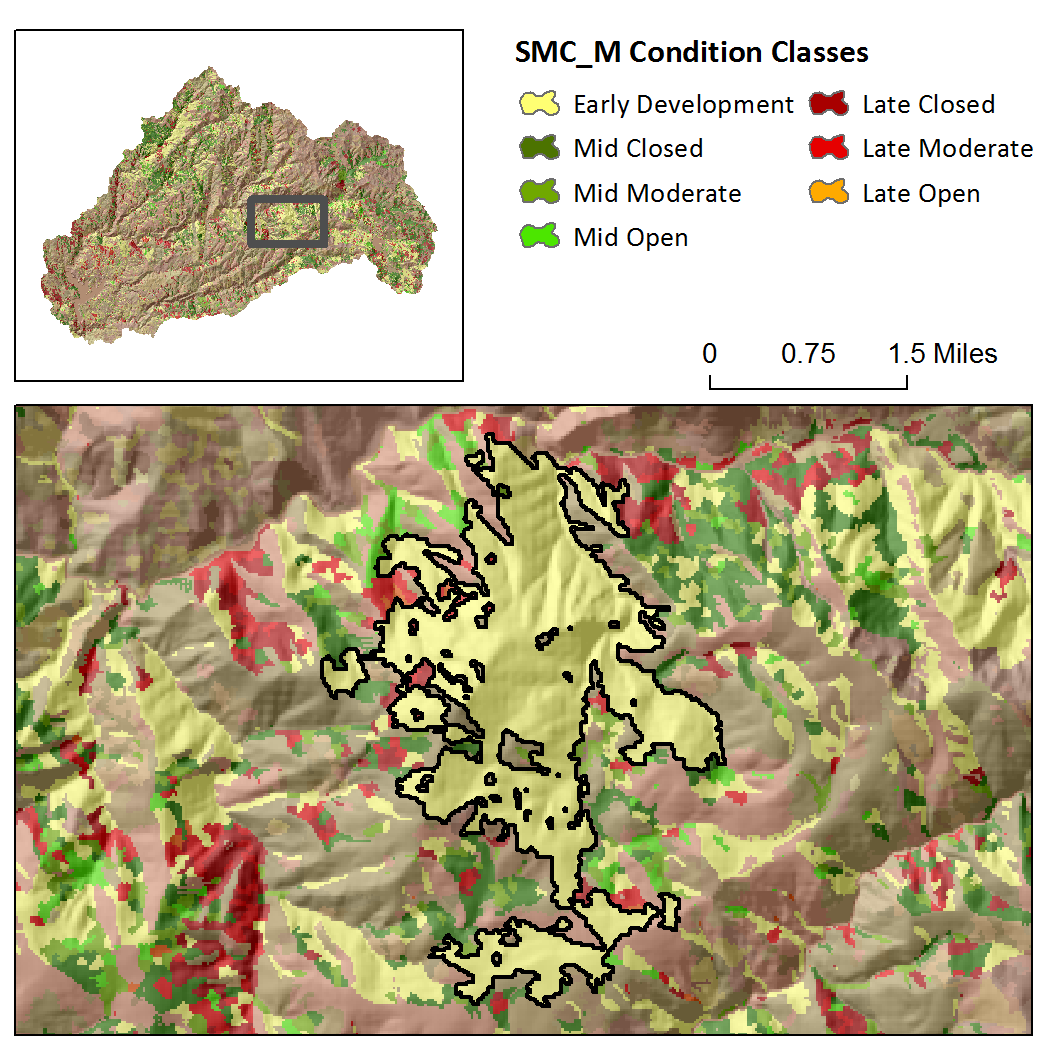
\includegraphics[width=0.5\textwidth]{/Users/mmallek/Tahoe/Report2/images/695_large_ED.png}
    \label{fig:patchmaps1-early}
    }%
  \subfloat[][]{
    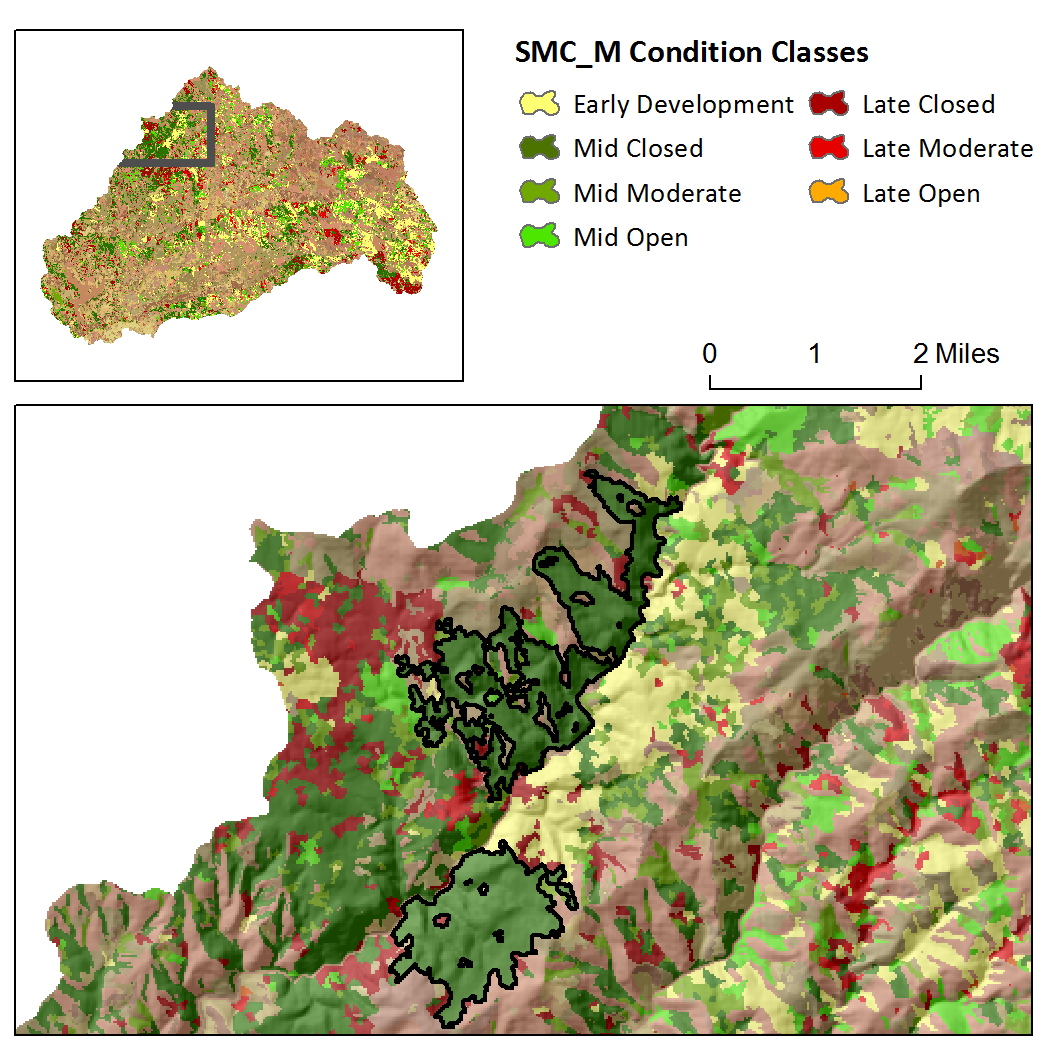
\includegraphics[width=0.5\textwidth]{/Users/mmallek/Tahoe/Report2/images/515_largeMD_2patches.png}
    \label{fig:patchmaps1-mid}
    }
  \caption{(a) A very large patch of Sierran Mixed Conifer - Mesic in Early Development during timestep 695. The patch highlighted with a dark black outline is 1,215 hectares, which is the second-largest patch during this timestep. (b) Two patches of Sierran Mixed Conifer - Mesic in Mid Development - Closed. These are two of the largest patches (in the top 25 out of over 40,000 patches) during timestep 515.} 
  \label{fig:patchmaps1}
\end{figure}

In addition, we observe increased dominance by certain cover-condition types, as illustrated by smaller values for the \emph{Simpson's Evenness Index} during the HRV (Figure~\ref{fig:fragland_contagsiei}). For example, within the Sierran Mixed Conifer - Xeric cover type, Early Development and Mid Development - Open were much more widespread during the simulated HRV than in the current landscape (Figure~\ref{fig:patchmaps2}). Because Sierran Mixed Conifer - Xeric is so widespread, this shift would directly influence \emph{Simpson's Evenness}, lowering its value.

\begin{figure}[!htbp]
  \centering
  \subfloat[][]{
    \centering
    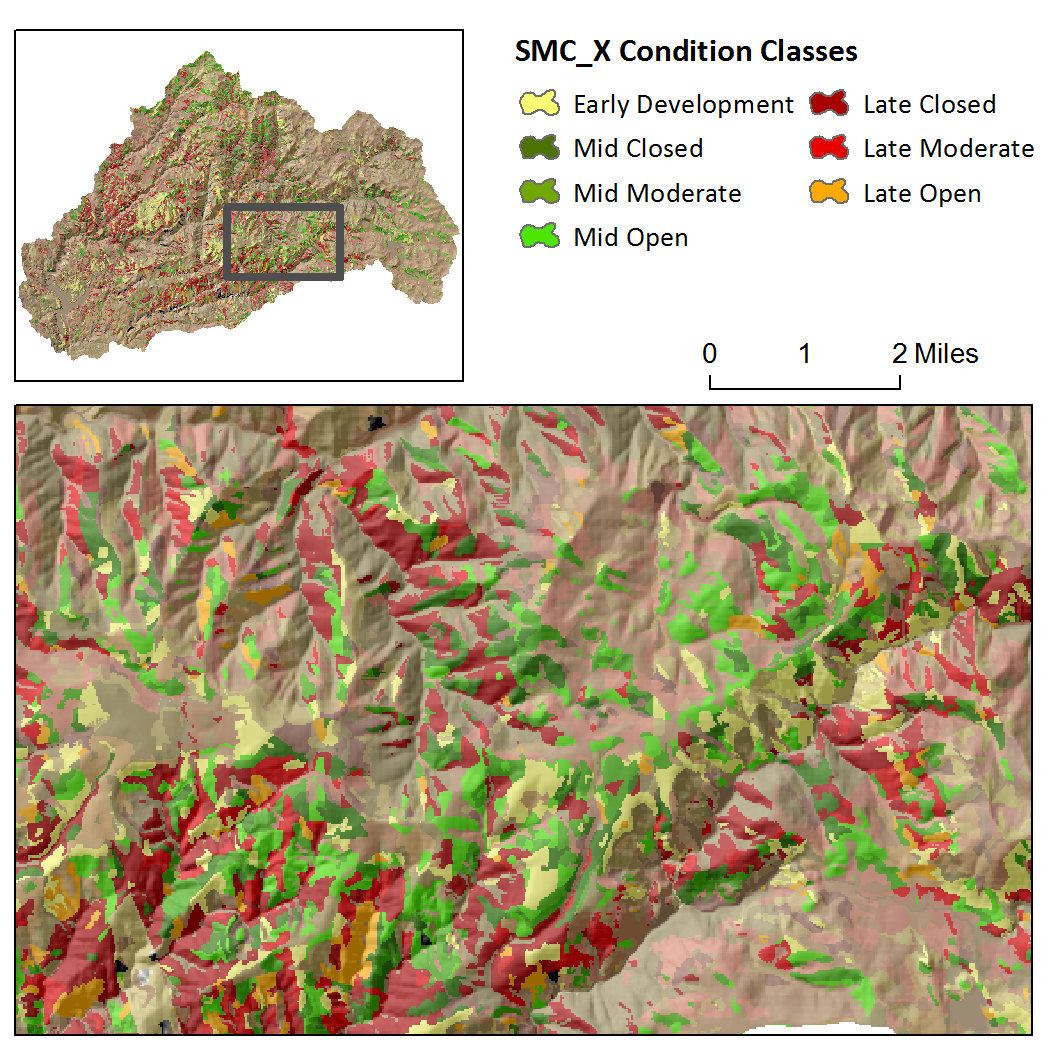
\includegraphics[width=0.45\textwidth]{/Users/mmallek/Tahoe/Report2/images/ts0_smcx_match570.png}
    \label{fig:patchmaps2-ts0}
    }%
  \subfloat[][]{
    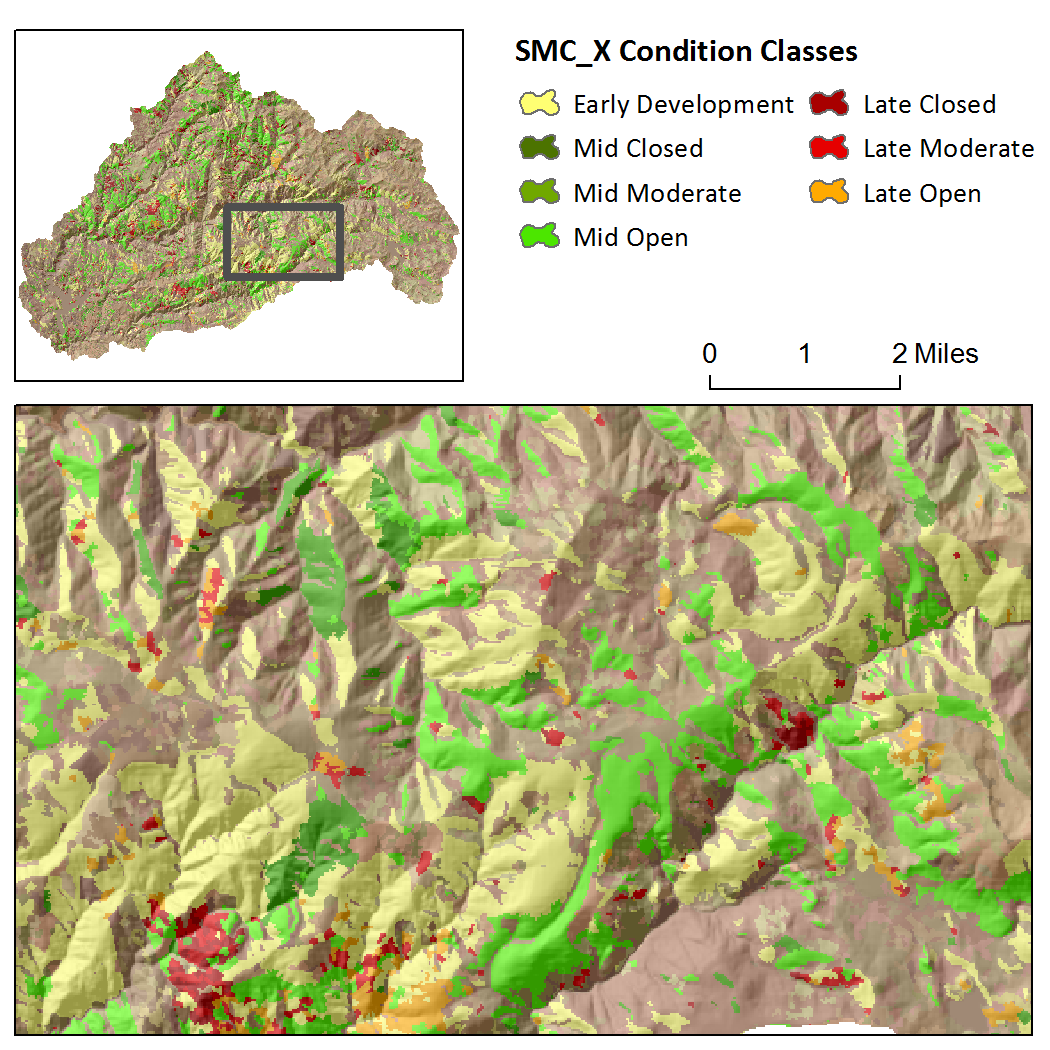
\includegraphics[width=0.45\textwidth]{/Users/mmallek/Tahoe/Report2/images/570_smcx_largeEDMD.png}
    \label{fig:patchmaps2-ts570}
    }
  \caption{Cover-Condition map focused on patches from Sierran Mixed Conifer - Xeric, showing increased dominance by certain cover-condition types during the HRV. (a) The current landscape. (b) The same region of the map during timestep 570. Note the contrast between the two maps with respect to the condition classes and size of individual patches.} 
  \label{fig:patchmaps2}
\end{figure}


Third, we find that patches on the landscape were more aggregated at the cell-level during HRV, which is illustrated by the \emph{Contagion} metric. In general, patches have low levels of both dispersion and interspersion. Of course, there are many ``edgy'' areas on the landscape, but this metric indicates that across the full landscape aggregation is more typical, particularly in comparison to the current landscape. Again, the homogeneity of post-fire early development stands likely aids in increasing the contagion value (Figure~\ref{fig:patchmaps3}). 

\begin{figure}[!htbp]
  \centering
  \subfloat[][]{
    \centering
    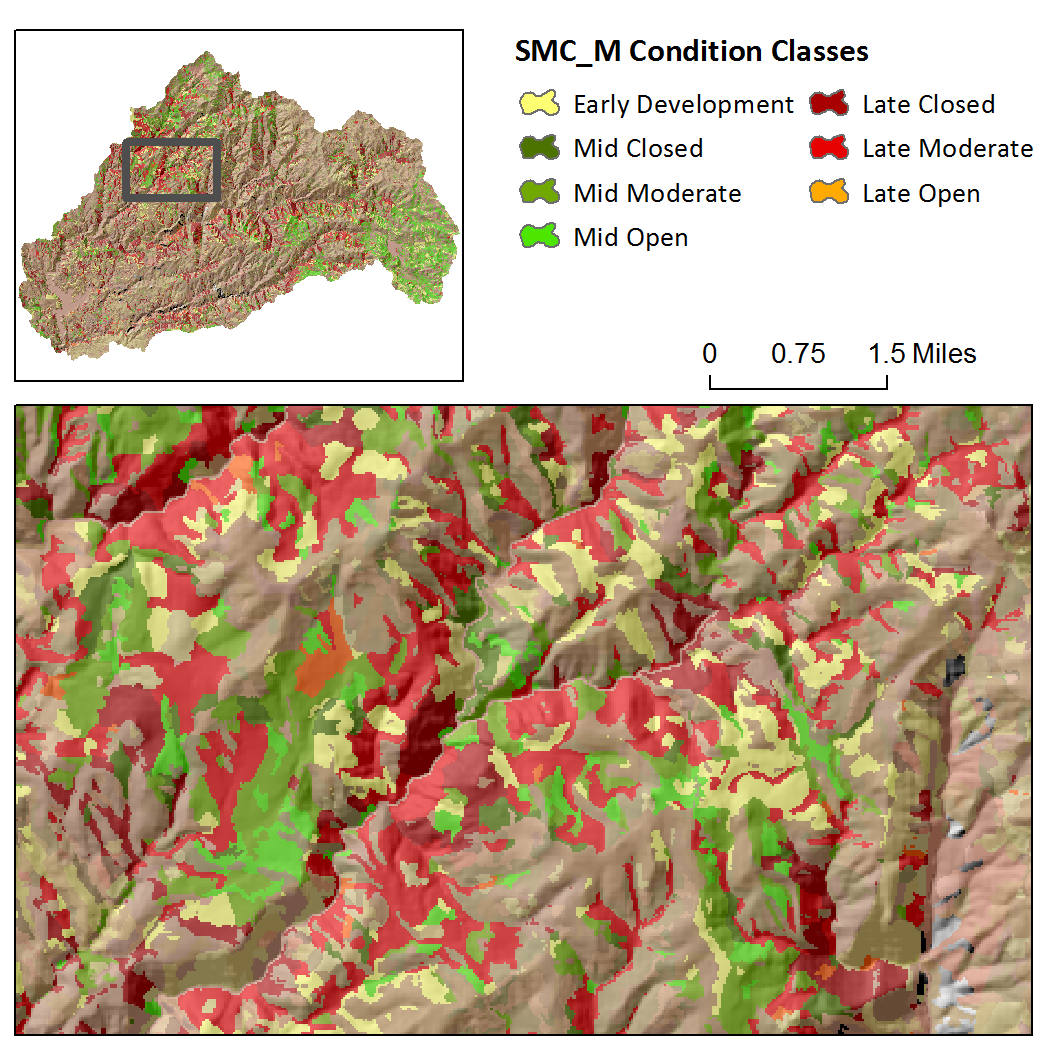
\includegraphics[width=0.45\textwidth]{/Users/mmallek/Tahoe/Report2/images/615_ts0_contag.png}
    \label{fig:patchmaps3-ts0}
    }%
  \subfloat[][]{
    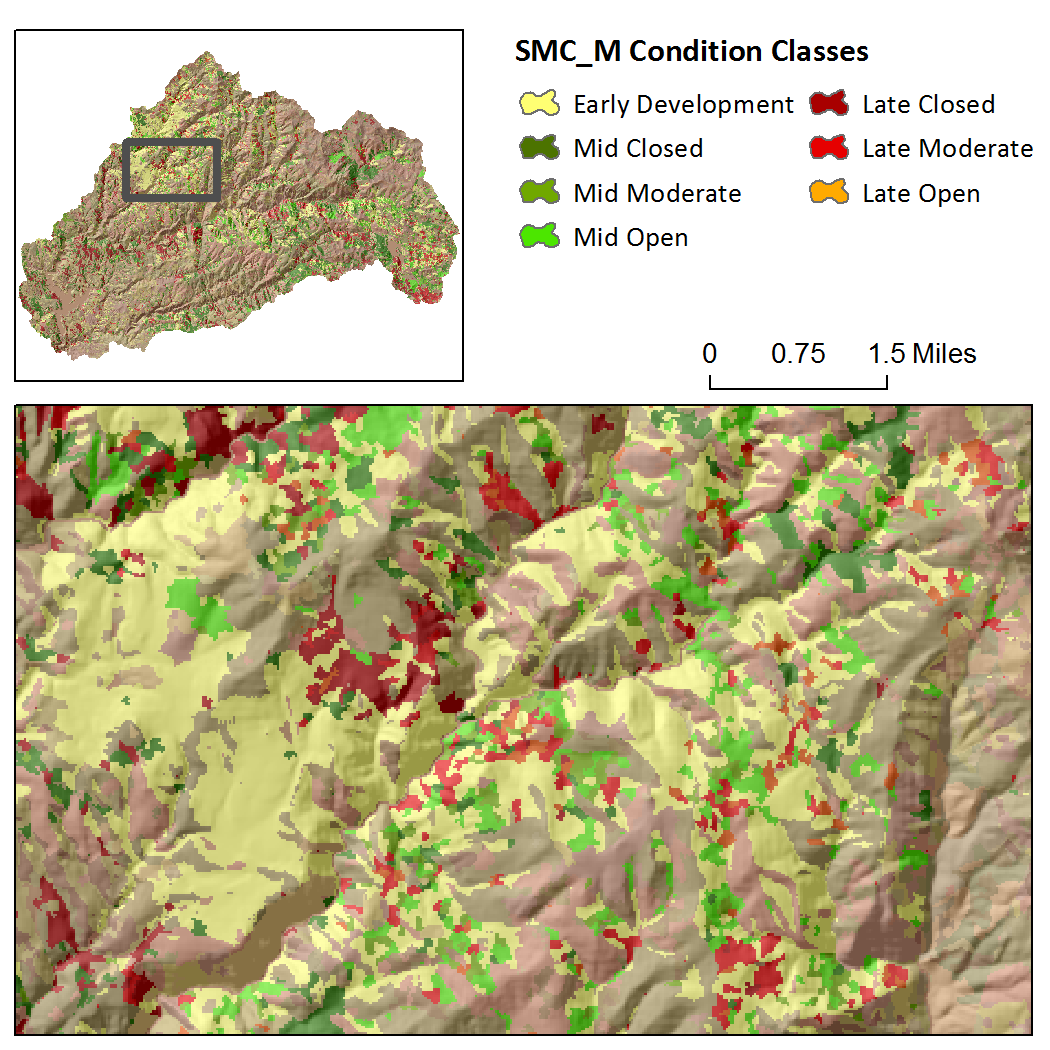
\includegraphics[width=0.45\textwidth]{/Users/mmallek/Tahoe/Report2/images/615_contag.png}
    \label{fig:patchmaps3-ts615}
    }
  \caption{Cover-Condition map focused on patches from Sierran Mixed Conifer - Mesic. (a) The current landscape. (b) The same region of the map during timestep 615. Note the contrast between the two maps with respect to the contagion (at the cell level).} 
  \label{fig:patchmaps3}
\end{figure}

However, despite being larger, more extensive, and aggregated, they do not show an associated increase in core area (Figure~\ref{fig:fragland_core}). This indicates that they are geometrically more complex, to the extent that little core area fits inside each patch. The results for the landscape metric \emph{Shape} confirm this analysis (Figure~\ref{fig:fragland_areashape}). Especially among the largest patches on the landscape, convoluted shapes are common. Again, this is not to say that large and simple shapes do not occur---they do---but in comparison to the current landscape, complex shapes were characteristic of the simulated HRV.

\begin{figure}[!htbp]
  \centering
  \subfloat[][]{
    \centering
    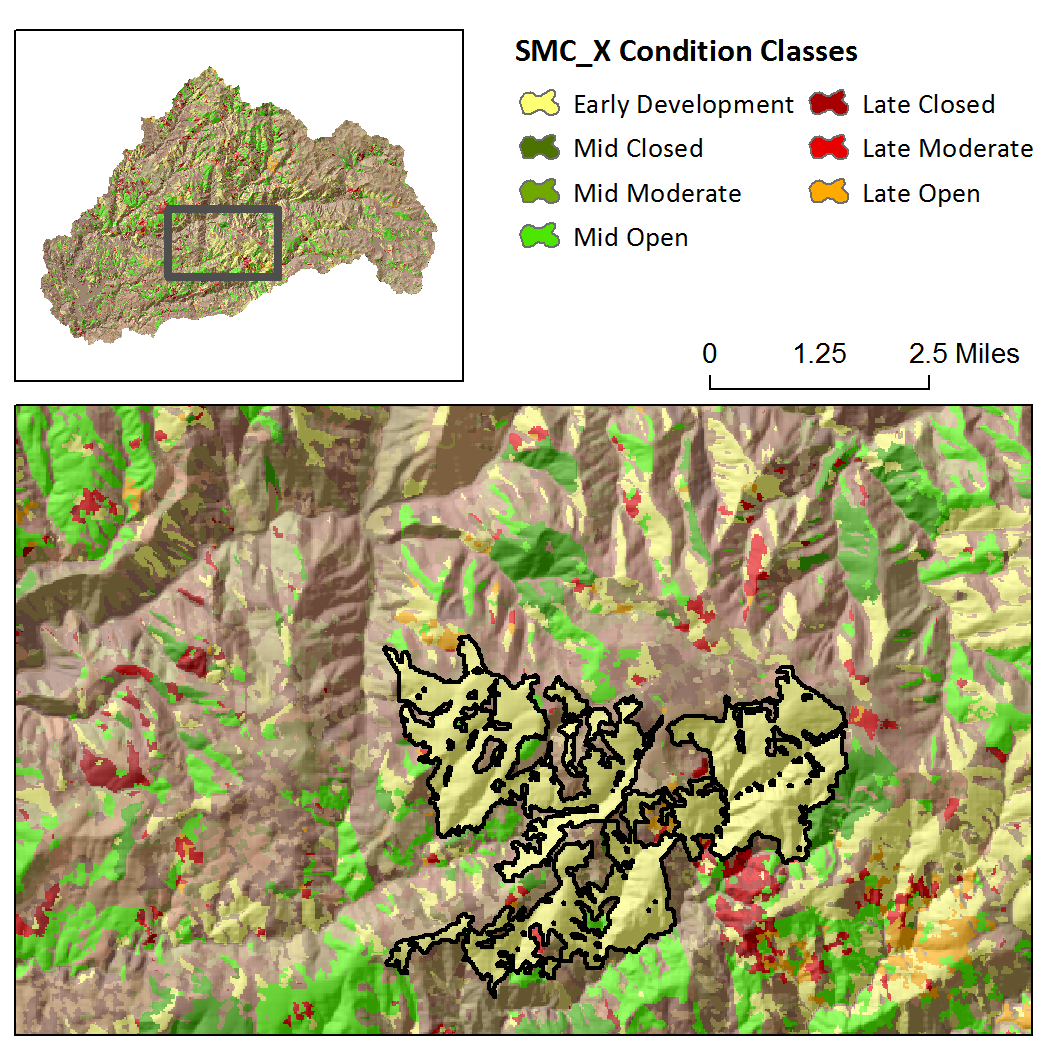
\includegraphics[width=0.45\textwidth]{/Users/mmallek/Tahoe/Report2/images/555_convoluted.png}
    \label{fig:patchmaps4-ts555}
    }%
  \subfloat[][]{
    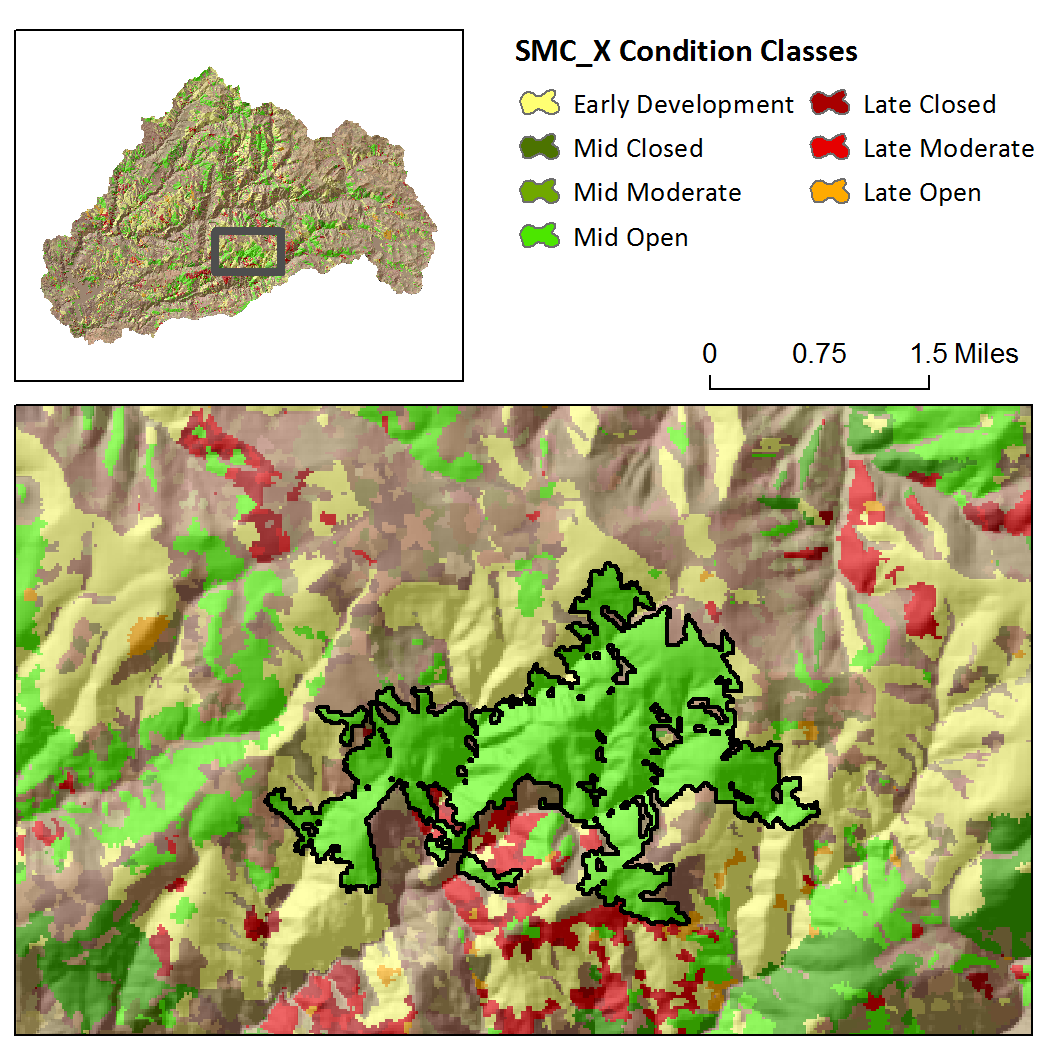
\includegraphics[width=0.45\textwidth]{/Users/mmallek/Tahoe/Report2/images/690_less_convoluted.png}
    \label{fig:patchmaps4-ts690}
    }
  \caption{Cover-Condition map focused on patches from Sierran Mixed Conifer - Xeric. (a) A large patch (2059 ha) from timestep 555 has little room is available for cores due to its irregular shape. (b) A large patch (828 ha) from timestep 690 is less geometrically complex, and thus has relatively more \emph{core area}.} 
  \label{fig:patchmaps4}
\end{figure}

\clearpage
\section{Management Implications}
%"Drawing comparisons between past and current fire frequencies can assist resource managers in prioritizing areas for ecological restoration, fuels reduction, certain fire or habitat management practices, and other activities. " (Hugh)

The primary goal of this study was to use our knowledge and understanding of vegetation dynamics and disturbance processes to simulate changes to landscape composition and configuration over time under a historical reference framework. We then compared those dynamics to observations of current conditions, and assessed the departure from the historic range of variability. Our landscape-level assessment is that both composition and configuration deviate substantially from the HRV. In general, the current landscape is dominated by Mid and Late Development forest and lacks the fire-dependent stand conditions (e.g. open canopy forest) and spatial heterogeneity in vegetation that were maintained by natural disturbances during the reference period. This landscape condition appear to be largely a legacy of the last 150 years of land management practices, especially fire suppression and timber management \citep{Safford2014,Stephens2007}. Substantial changes to the ecology and landscape function in western forest landscapes have been documented not only in the Sierra Nevada, but also in the Cascades and Rocky Mountains \citep{Hessburg2005,Baker2012,Baker2014,Mallek2013,Agee1993} . However, little research has been done that incorporates spatially explicit disturbance and succession modeling in combination with analyses of landscape structure.\todo{Kevin do you think the last sentence is accurate?}

In the western Sierra Nevada, foothill communities and lower elevation oak-conifer woodlands have experience a loss of species diversity, fragmentation, and outright habitat conversion due to the overlap with private lands and population growth. Middle elevation forests were and are more affected by mining and forestry; most easily accessible trees were probably cut before national forests were established \citep{SNEP1996}. The wildfire regime has been significantly altered in hardwoods, yellow pine, and mixed conifer forests \citep{Merriam2013,Safford2013}, and much less so in red fir and subalpine forests \citep{Meyer2013,Meyer2013a}. However, other human activities since the late 1800s have altered the structure of western Sierra Nevada forests, most notably to simplify it in several ways, including a decrease in species, multi-story canopies, and snags \citep{SNEP1996}. These activities are related mainly to timber harvest and to the extensive network of roads constructed to support timber harvest, fire control, and recreation. It has been suggested that this simplification of landscape structure may have a negative impact on wildlife and potentially lead to a loss of biodiversity in forests \citep{Thompson2003,Manley2004,Hunter2011}. Isolating the effect of fragmentation in our study landscape is made more difficult due to the inherent heterogeneity of Sierran landscapes---a consequence of steep natural gradients in elevation, topography, and substrate---and forests in this region tend to be somewhat patchy even in the absence of human alterations \citep{Franklin1996}. In the Pacific Northwest, ``old-growth'' connotes very large blocks of uniformly very old trees. However, in the Sierra Nevada ``old-growth'' indicates not only the presence of very large and old trees, but also a complex, patchy, ``messy'' forest of varying age classes, species, fuel quantities, and vegetation structure \citep{SNEP1996}.

% don't think climate was benign in the SN during recent past - after settlement there was a lot of mining, a lot of harvest, and a lot of fire. fire slowed down when suppression began. 
% Forest fragmentation in the sierra nevada
% changes to plants and animals from fire suppression, logging, road-building
% included Spotted Owl and Northern Goshawk!!
% logging removes habitat that would be used by birds, true for salvage also (Cahall and Hayes 2008)
% roads are bad - show map with roads (Gucinski et al. 2001)
% would not say we are in early stages of understanding fragmentation
% late successional very important - Franklin et al. Alternative Approaches, call for 5-30k acre patches (run fragstats on the rec4 without special tables?)


% omitting this paragraph - not sure it's relevant
%\paragraph{p2}Our findings are particularly interesting in light of increasing concern over anthropogenic habitat loss and fragmentation (Rochelle et al. 1999; Knight et al. 2000). Forest fragmentation has received considerable research attention in many regions of North America (e.g., Whitcomb et al. 1981; Robbins et al. 1989; Lehmkuhl and Ruggiero 1991; McGarigal and McComb 1995; Schmiegelow et al. 1997; Trzcinski et al. 1999; Villard et al. 1999). %Girvetz eta al. 2008 (California). However, we are in the earliest stages of understanding the patterns, processes, and ecological significance of forest fragmentation in the southern Rocky Mountain region (Knight et al. 2000). It is not clear, for example, how the native biota responds to anthropogenic changes in landscape patterns caused by logging and road-building and disruption of natural disturbance regimes (e.g., fire suppression). 



Based on our results, it might be tempting for managers to reach the simple conclusion that the landscape is less fragmented today than during the reference period. For example, today's landscape is simpler (lower \textsc{shape} values), contains less core area (based on \textsc{core\_am}), and has less contrast between patch types (\textsc{econ\_am}). However, this conclusion is not as straightforward as it might seem. Fragmentation is a landscape-level process in which a specific habitat is progressively sub-divided into smaller, geometrically altered, and more isolated fragments as a result of both natural and human activities. This process involves changes in landscape composition, structure, and function at many scales and occurs on a backdrop of a natural patch mosaic created by vegetation transitions, both those mediated by and independent from natural disturbances \citep{McGarigal1995}. The scale at which fragmentation occurs is at the level of a specific habitat type; it is the habitat, rather than the landscape, that becomes fragmented. In this study we evaluated the spatial pattern---and by implication, the fragmentation---of many different patch types (defined by unique combinations of cover type and condition class). Certaintly, some of these patch types are less fragmented in the current landscape than they were under the simulated HRV. 

% Taking this out because adding an analysis of clumped "late" or "mid" is a lot of extra work. Probably beyond scope right now; could be part of phase II if this happens (language would be to revise HRV analysis and future scenarios analysis to include groupings - could take this in several directions, such as lumping the mesic and xeric types together for analysis also.)
%\todo{Need help with script to evaluate stages by themselves}\emph{This is true in general for most of the late-seral forest patch types. However, not all patch types are less fragmented in the current landscape. For example, many of the early-seral forest patch types are in fact much more fragmented in the current landscape than they were under the simulated HRV.} Thus, conclusions about habitat fragmentation in the current landscape must be qualified with specific reference to one or more well-defined habitats.

In addition, we evaluated vegetation patterns in the current landscape after excluding roads (i.e., we removed roads from the land cover map by filling in those areas with the nearest alternate cover type). Figure \ref{fig:roadcovermap} shows the cover type layer with roads overlaid. %
%
\begin{figure}[!htbp]
  \centering
  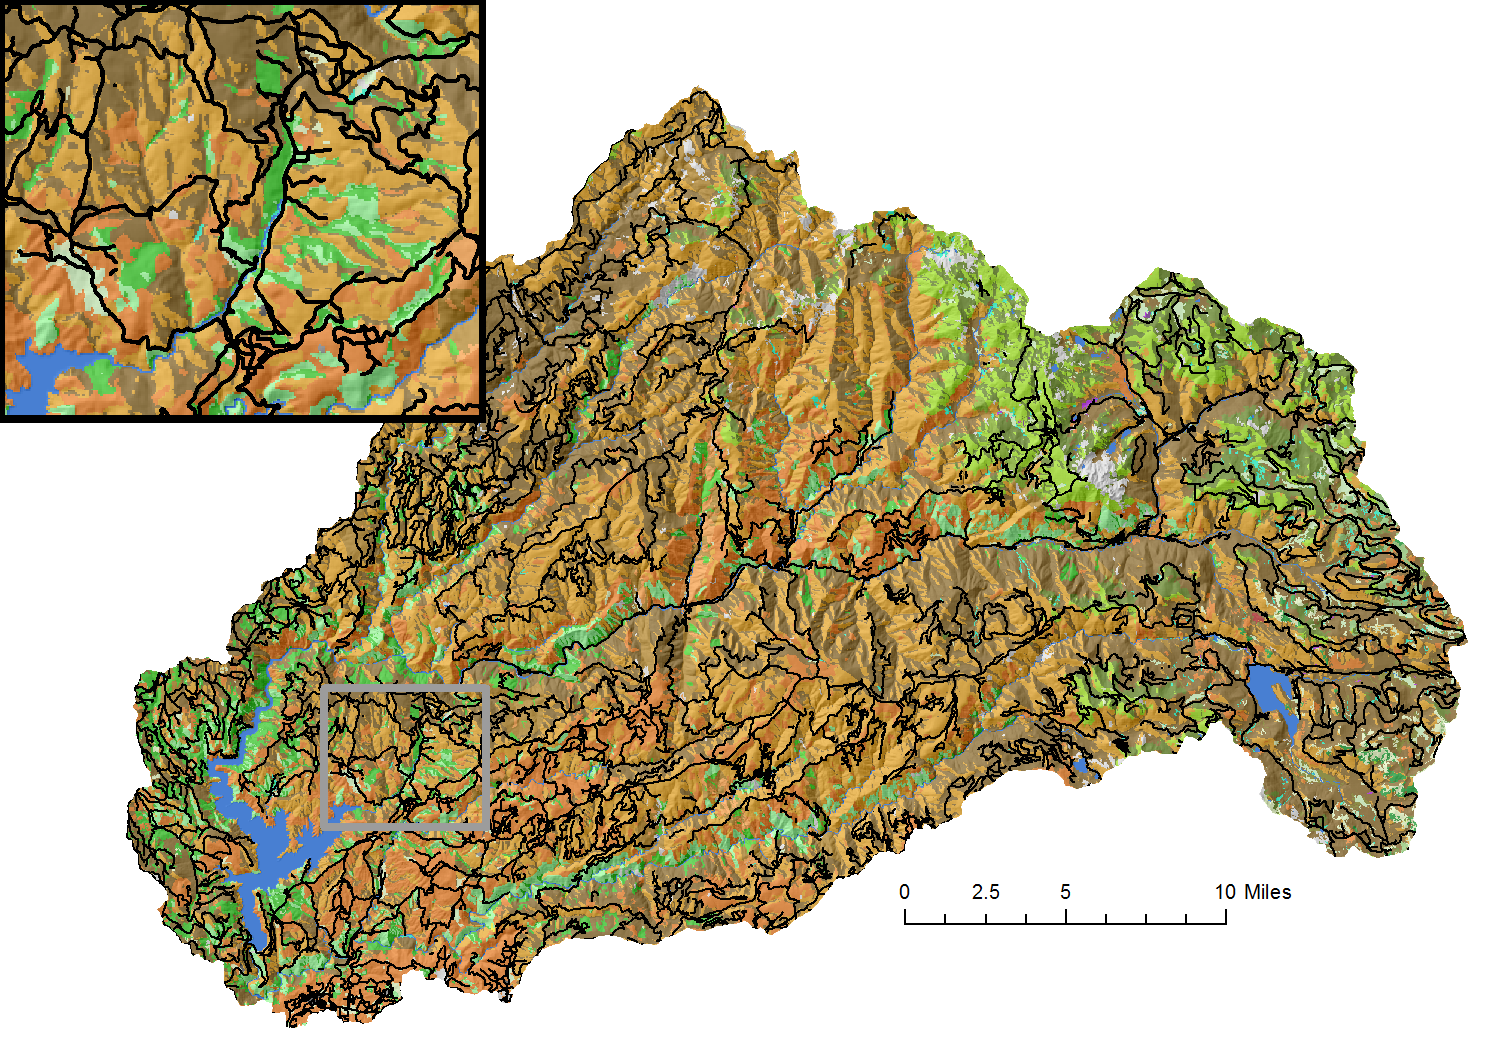
\includegraphics[height=.4\textheight]{/Users/mmallek/Tahoe/Report2/images/roads_cover.png}
  \caption{The core project area superimposed with the cover type map and all roads in black. There are a two designated roadless areas, but in general roads are common throughout the watershed. The closeup area is just northeast of the Pendola reservoir.} 
  \label{fig:roadcovermap}
\end{figure}
%
We did this in order to be consistent with our simulation of landscape structure changes during the reference period. However, the significant and extensive impact of roads on Sierran ecosystems is well documented in the literature \citep{Karr2004,Trombulak2000,Gucinski2001,Theobald2011}.  In particular, roads are linear landscape features that can create high-contrast edges and bisect patches. They may cause greater fragmentation of habitats than the direct loss of habitat from associated land use activities \citep{Gucinski2001,Tinker1998,Mcgarigal2001}. Given the large amount of roads within the project area and their disproportionate influence on landscape structure and function, any conclusions regarding departure in relation to habitat fragmentation that does not consider road impacts should be viewed with extreme caution. The impacts of roads on landscape structure will be addressed in our evaluation of alternative land management scenarios in the next phase of this project\todo{Keep this last sentence?}.

%"Drawing comparisons between past and current fire frequencies can assist resource managers in prioritizing areas for ecological restoration, fuels reduction, certain fire or habitat management practices, and other activities. " (Hugh)

Our results imply that any attempt to restore the landscape structure to a composition and configuration that aligns with the historic range of variability described in this report would likely be a difficult and long-term undertaking, if it were deemed desirable or even possible. Our model equilibration period is the length of the interval between the starting condition and structure (in this case, of the current landscape) and beginning of a stable range of variation. It is a function of not only how far outside the stable range of variation the current landscape is, but also the speed at which disturbance and succession processes interact to affect a change in the landscape trajectory. Thus, we can infer that if management activities were designed to emulate natural disturbance processes, then it would take a length of time equal to the equilibration period to return the landscape to its HRV. The equilibration period for our simulation was 40 timesteps, or 200 years. Given that forest planning horizons are on timescales of 5--30 years, and the fact that climate change is predicted to have measurable impacts on both wildfires and vegetation community succession and structure over the next several decades, an effort to ``restore'' the current landscape to the conditions aligning with our simulated HRV is impractical. Moreover, the extent and intensity of disturbance required to emulate the natural disturbance regime would be unacceptable socially, economically, and politically. However, as several ecologists have pointed out, it may be appropriate to use our results for prioritizing areas for restoration, designing fire and fuels management projects, or setting goals for future trajectories of forest structure \citep{Safford2013,Keeley2000}.

\section{ NEW DRAFT RECOMMENDATIONS - IN PROGRESS}
\section{Individual Cover Type Recomendations}
Our study methodology makes it possible to single out separate cover types and condition classes for analysis, and in this section we provide some interpretation of those results that is targeted toward providing recommendations for specific strategies that could be used to push landscape structure toward the HRV, and other recommendations of management strategies to avoid. Because in reality cover types are interspersed with one another, managers will need to consider the recommendations for individual cover types within the context of the vegetation actually present within a given management unit.

\subsection{Mixed Evergreen - Mesic}
Mesic mixed evergreen forests are thought to have burned with a fire rotation of 63 years under historical conditions. Low mortality fire was much more common than high mortality fire, but both are necessary to create stand structure and composition similar to that observed during the simulation. Late development stands of mixed evergreen were relatively uncommon during the simulation, especially compared to the current landscape. The current landscape also contains more area in the Early Development condition (Figure \ref{fig:covcondbar_megm}. Based on these observations, we recommend management strategies that imitate low-mortality disturbance; that is, removing less than 70\% of the existing top-level canopy cover. Such a strategy would provide a mechanism for the forest to age into the late development conditions. It is not necessary for all stands of mesic mixed evergreen forests to receive the same treatment on the same schedule. In certain parts of the forest, fires would have recurred more frequently than the 63 year rotation (see Figure \ref{fig:preturn_megm}). The grand mean fire return interval for low mortality fires within this cover type ranged\todo{best way to phrase this??} from around 25 years to 100 years. Managers who are charged with focusing fuels reduction on certain areas within the forest could set goals of carrying out vegetation treatments somewhat more frequently in certain parts of the forest and less frequently in other parts, thereby also contributing to the overall more complex landscape pattern observed during the simulated HRV. 

\begin{figure}[!htbp]
  %\centering
  \subfloat[][]{
    \centering
    \includegraphics[width=0.8\textwidth]{/Users/mmallek/Tahoe/Report2/images/CovcondHRVBarplots/MEGM_Early_AllStructures_srvplot.pdf}
  }\\%
  %\subfloat[][]{
    \centering
    \includegraphics[width=0.8\textwidth]{/Users/mmallek/Tahoe/Report2/images/CovcondHRVBarplots_nolegend/MixedEvergreen-Mesic_Mid-Closed_srvplot.pdf}
  }\\%
  %  \subfloat[][]{
    \centering
    \includegraphics[width=0.8\textwidth]{/Users/mmallek/Tahoe/Report2/images/CovcondHRVBarplots_nolegend/MixedEvergreen-Mesic_Mid-Moderate_srvplot.pdf}
  }\\%
  %  \subfloat[][]{
    \centering
    \includegraphics[width=0.8\textwidth]{/Users/mmallek/Tahoe/Report2/images/CovcondHRVBarplots_nolegend/MixedEvergreen-Mesic_Mid-Open_srvplot.pdf}
  }\\%
  %  \subfloat[][]{
    \centering
    \includegraphics[width=0.8\textwidth]{/Users/mmallek/Tahoe/Report2/images/CovcondHRVBarplots_nolegend/MixedEvergreen-Mesic_Late-Closed_srvplot.pdf}
  }\\%
  %  \subfloat[][]{
    \centering
    \includegraphics[width=0.8\textwidth]{/Users/mmallek/Tahoe/Report2/images/CovcondHRVBarplots_nolegend/MixedEvergreen-Mesic_Late-Moderate_srvplot.pdf}
  }\\%
  %  \subfloat[][]{
    \centering
    \includegraphics[width=0.8\textwidth]{/Users/mmallek/Tahoe/Report2/images/CovcondHRVBarplots_nolegend/MixedEvergreen-Mesic_Late-Open_srvplot.pdf}
  }\\%
  \caption{Cover-condition barplots for Mixed Evergreen - Mesic dynamics. For each condition class, the color the bar represents the distance from the median value during the simulated HRV. Green represents the 25th-75th percentiles; yellow represents the 5th-25th and 75th to 95th percentiles; red represents the 0th-5th and 95th-100th percentiles. The blue vertical line marks the 50th percentile and the black vertical line indicates the current cover extent. To read the ``Early–All Structures'' barplot, for a given percentage of the cover type extent, the x-axis value indicates an observed proportion, and the color corresponding to that point indicates the percentile range that value falls within. In this example, the current percent of cover extent for this cover type and condition class falls within the 95th-100th percentile range during the simulated HRV.}
  \label{fig:covcondbar_megm}
\end{figure}

With respect to the landscape structure metrics (computed using \textsc{Fragstats}), we highlight the values for the Late Development - Closed and Moderate conditions, since they dominated during the HRV simulation. We observed that present-day patches of mesic mixed evergreen forests in these conditions were smaller, more clumped, less geometrically complex, and contained less core area than during the simulated HRV. Having less core area and being more clumped may seem contradictory, but this outcome is likely due to the smaller size of the current patches. Restoration of these forests to patches that reflect a more natural succession process may be challenging for managers, given practical needs like using roads and riparian buffers as the edges of treatment units. It may not be practical to perform mechanical treatments over large areas within this cover type. However, when conducting treatments using prescription fires, creative solutions should be sought to generate more complex edges and to complete burns over sufficiently large areas that larger core areas can be generated.

Because the most commonly occuring condition classes for mesic mixed forests were actually late development closed and moderate canopy cover, it may also be more helpful for managers to think about this cover type not as receiving direct treatment, but as being influenced by other treatments targeting cover types such as oak-conifer forests and woodlands or sierran mixed conifer forests. When mesic mixed evergreen forests border or serve as the edge of treatment units targeting other vegetation types, managers can evaluate the patches of mesic mixed evergreen forests present at the time of treatment and consider whether to expand the management unit to treat them, to try and achieve an irregular edge to increase patch complexity, or to exclude them from treatment in order to promote development into the late development conditions.                                                                                                                                                                                                                                                                                                                                                                                                                                                    












